\documentclass[a4paper]{article}
\usepackage[warn]{mathtext} %для поддержки кириллицы в формулах
\usepackage{amsmath} %основной пакет для формул
\usepackage[utf8x]{inputenc}
\usepackage[T1,T2A]{fontenc}
\usepackage[russian]{babel}
\usepackage{hyperref}
\usepackage{indentfirst}
\usepackage{listings}
\usepackage{color}
\usepackage{xcolor}
\usepackage{here}
\usepackage{array}
\usepackage{multirow}
\usepackage{graphicx}

\definecolor{linkcolor}{HTML}{000000} % цвет ссылок 000000 = чёрный
\definecolor{urlcolor}{HTML}{0000FF} % цвет гиперссылок 0000FF = синий
 
\hypersetup{pdfstartview=FitH, pagecolor=black, linkcolor=linkcolor,urlcolor=urlcolor, colorlinks=true}
\usepackage{caption}

\renewcommand{\lstlistingname}{Программа} % заголовок листингов кода

\usepackage{listings}
\lstset{ %
extendedchars=\true,
keepspaces=true,
language=c++,					% choose the language of the code
basicstyle=\footnotesize,		% the size of the fonts that are used for the code
numbers=left,					% where to put the line-numbers
numberstyle=\footnotesize,		% the size of the fonts that are used for the line-numbers
stepnumber=1,					% the step between two line-numbers. If it is 1 each line will be numbered
numbersep=5pt,					% how far the line-numbers are from the code
backgroundcolor=\color{white},	% choose the background color. You must add \usepackage{color}
showspaces=false				% show spaces adding particular underscores
showstringspaces=false,			% underline spaces within strings
showtabs=false,					% show tabs within strings adding particular underscores
frame=single,           		% adds a frame around the code
tabsize=2,						% sets default tabsize to 2 spaces
captionpos=b,					% sets the caption-position to bottom
breaklines=true,				% sets automatic line breaking
breakatwhitespace=false,		% sets if automatic breaks should only happen at whitespace
escapeinside={\%*}{*)},			% if you want to add a comment within your code
postbreak=\raisebox{0ex}[0ex][0ex]{\ensuremath{\color{red}\hookrightarrow\space}}
}

\usepackage[left=2cm,right=2cm,
top=2cm,bottom=2cm,bindingoffset=0cm]{geometry}

\newcommand{\RomanNumeralCaps}[1]
    {\MakeUppercase{\romannumeral #1}}

\begin{document}	% начало документа

\begin{titlepage}	% начало титульной страницы

	\begin{center}		% выравнивание по центру

		\large Санкт-Петербургский Политехнический Университет Петра Великого\\
		\large Институт компьютерных наук и технологий \\
		\large Кафедра компьютерных систем и программных технологий\\[6cm]
		% название института, затем отступ 6см
		
		\huge Программирование\\[0.5cm] % название работы, затем отступ 0,5см
		\large Курсовой проект по программированию\\[0.1cm]
		\large Игра Шахматы\\[5cm]

	\end{center}


	\begin{flushright} % выравнивание по правому краю
		\begin{minipage}{0.25\textwidth} % врезка в половину ширины текста
			\begin{flushleft} % выровнять её содержимое по левому краю

				\large\textbf{Работу выполнил:}\\
				\large Крылов И.С.\\
				\large {Группа:} 13501/4\\
				
				\large \textbf{Преподаватель:}\\
				\large Вылегжанина К.Д.

			\end{flushleft}
		\end{minipage}
	\end{flushright}
	
	\vfill % заполнить всё доступное ниже пространство

	\begin{center}
	\large Санкт-Петербург\\
	\large \the\year % вывести дату
	\end{center} % закончить выравнивание по центру

\thispagestyle{empty} % не нумеровать страницу
\end{titlepage} % конец титульной страницы

\vfill % заполнить всё доступное ниже пространство



% Содержание
\hypertarget{toc}
\tableofcontents
\newpage



\section*{Шахматы}
\addcontentsline{toc}{section}{Глава 1. Шахматы}

\textbf{Шахматы} - всемирно известная логическая стратегическая игра, впервые возникшая в Индии полторы тысячи лет назад. Данная игра развивает логическое мышление, официально признана видом спорта и является одной из самых популярных настольных игр.

\subsection*{Задание}
\addcontentsline{toc}{subsection}{Задание}
Графическое представление шахматного поля с возможностью перемещать фигуры в соответствии с правилами, предусмотренными игрой.\\
Реализация игры шахматы с графическим интерфейсом и предусмотренным искусственным интелектом. Возможность изменять начальные параметры игры.\\
\subsection*{Концепция}
\addcontentsline{toc}{subsection}{Концепция}
Реализация игры шахматы: графическое представление поля, фигур, возможность перемещать шахматные фигуры по полю в соответствии с правилами, предусмотренными игрой. Несколько режимов игры на выбор: игра со вторым пользователем и игра с искуственным интелектом. Реализация искуственного интелекта на уровне случайных неанализируемых ходов, не противоречащим правилам игры, и на уровне анализируещего механизма, целью которого является нахождение наиболее выгодной стратегии для победы. Возможность изменять предустановки игры: выбор цвета фигур, опциональная возможность играть с/без счётчика времени. Тем самым пользователю предоставляется виртуальная реализация настольной игры шахматы.\\

\subsection*{Правила игры}
\addcontentsline{toc}{subsection}{Правила игры}

\subsubsection*{Доска и начальная позиция}
\addcontentsline{toc}{subsubsection}{Доска и начальная позиция}
 Игра происходит на доске, поделенной на равные квадратные клетки, или поля. Размер доски — 8×8 клеток. Вертикальные ряды полей (вертикали) обозначаются латинскими буквами от а до h слева направо, горизонтальные ряды (горизонтали) — цифрами от 1 до 8 снизу вверх; каждое поле обозначается сочетанием соответствующих буквы и цифры. Поля раскрашены в тёмный и светлый цвета (и называются, соответственно, чёрными и белыми) так, что соседние по вертикали и горизонтали поля раскрашены в разные цвета. Доска располагается так, чтобы ближнее угловое поле справа от игрока было белым (для белых это поле h1, для черных — поле а8). У игроков в начале игры имеется по одинаковому набору фигур. Фигуры одного из игроков условно называются «белыми», другого — «чёрными». Белые фигуры окрашены в светлый цвет, чёрные в тёмный. Сами игроки называются «белые» и «чёрные» по цвету своих фигур.В каждый комплект фигур входят: король, ферзь, две ладьи, два слона, два коня и восемь пешек. В начальной позиции фигуры обеих сторон размещаются так, как показано на диаграмме. Белые занимают первую и вторую горизонтали, чёрные — седьмую и восьмую. Пешки расположены на второй и седьмой горизонталях соответственно.\\

\subsubsection*{Ходы}
\addcontentsline{toc}{subsubsection}{Ходы}
Игра заключается в том, что игроки поочерёдно делают ходы. Первый ход делают белые. За исключением взятия на проходе и рокировки, описанных ниже, ход заключается в том, что игрок перемещает одну из своих фигур на другое поле по следующим правилам:\\
\begin{itemize}
\item Фигуры, кроме коня, во время хода считаются передвигающимися по прямой линии в плоскости доски, то есть «проходящими» все поля между начальным и конечным, поэтому все эти поля должны быть свободны. Если на пути фигуры находится другая фигура, то переместить фигуру на поле за ней невозможно. Исключением является ход коня (см. ниже)\\
\item Ход на поле, занятое своей фигурой, невозможен\\
\item При ходе на поле, занятое чужой фигурой, она снимается с доски (взятие)\\
\item Король ходит на расстояние 1 по вертикали, горизонтали или диагонали\\
\item Ферзь ходит на любое расстояние по вертикали, горизонтали или диагонал\\
\item Ладья ходит на любое расстояние по вертикали или горизонтали\\
\item Слон ходит на любое расстояние по диагонали\\
\item Конь ходит на поле, находящееся на расстоянии 2 по вертикали и 1 по горизонтали или 1 по вертикали и 2 по горизонтали от текущего положения. В отличие от всех остальных шахматных фигур, ход коня делается вне плоскости доски, то есть конь непосредственно перемещается («перепрыгивает») с начального поля на конечное и никакие фигуры, стоящие на других полях, ходу коня помешать не могут. В частности, конь может ходить на поле, даже если оно полностью окружено своими или чужими фигурами\\
\item Пешка ходит со взятием по диагонали на одно поле вперёд-вправо или вперёд-влево, а без взятия — по вертикали на одно поле вперёд. Если пешка в данной партии ещё не делала ходов, она может сделать ход без взятия на два поля вперёд. Направлением «вперёд» называется направление к восьмой горизонтали для белых или к первой для чёрных. Когда пешка ходит на последнюю горизонталь (для белых — на восьмую, для чёрных — на первую), ходящий должен заменить её на любую другую фигуру того же цвета, кроме короля (превращение пешки). Превращение пешки является частью того хода, которым она перемещается на последнюю горизонталь. Таким образом, если, например, превращённая из пешки фигура угрожает королю противника, то этот король в результате хода пешкой на последнюю горизонталь немедленно оказывается под шахом\\
\end{itemize}
Кроме того, есть два специальных хода:
\begin{itemize}
\item Рокировка — если король и одна из ладей того же цвета не двигались с начала игры, то король и эта ладья могут в один ход одновременно сменить положение (рокироваться). При рокировке король сдвигается на 2 клетки по направлению к ладье, а ладья ставится на поле между начальной и конечной позицией короля. Рокировка невозможна, если король или соответствующая ладья уже ходили. Рокировка временно невозможна, если поле, на котором стоит король, или поле, которое он должен пересечь, или поле, которое он должен занять, находится под ударом одной из фигур противника, или если между рокируемыми королём и ладьёй находится какая-либо фигура. Рокировка считается ходом короля, а не ладьи, поэтому рокировку следует начинать с перестановки короля, а не ладьи\\
\item Взятие на проходе — когда пешка совершает ход на две клетки через битое поле, находящееся под ударом пешки противника, то ответным ходом она может быть взята этой пешкой противника. При этом пешка противника перемещается на битое поле, а сбитая пешка снимается с доски. Взятие на проходе возможно только непосредственно в ответ на ход пешки через битое поле, на следующих ходах оно уже не разрешено\\
\end{itemize}

\subsubsection*{Шах, мат и пат}
\addcontentsline{toc}{subsubsection}{Шах, мат и пат}
\begin{itemize}
\item[>] Король, находящийся на битом поле, называется стоящим под шахом. Сделать ход, после которого король противника оказывается под шахом, значит дать шах королю (или объявить шах). Ходы, после которых король сделавшего ход остаётся или оказывается под шахом, запрещены; игрок, король которого находится под шахом, обязан немедленно его устранить\\
\item[>] Если король игрока находится под шахом и игрок не имеет ни одного хода, позволяющего устранить этот шах, этот игрок называется получившим мат, а его противник поставившим мат. Цель игры и состоит в том, чтобы поставить мат королю противника\\
\item[>]  Если игрок при своей очереди хода не имеет возможности сделать ни одного хода по правилам, но король игрока не находится под шахом, такая ситуация называется пат\\
\end{itemize}

\subsubsection*{Итог игры}
\addcontentsline{toc}{subsubsection}{Итог игры}
Игра завершается выигрышем одной из сторон или ничьей.

Выигрыш фиксируется в следующих случаях:
\begin{enumerate}
\item Мат. Игрок, поставивший мат, выигрывает\\
\item Один из игроков сдался. Игрок, решивший, что дальнейшее сопротивление бессмысленно, может сдаться в любой момент. Его противник объявляется победителем\\
\end{enumerate}

Ничья фиксируется в следующих случаях:
\begin{enumerate}
\item Пат\\
\item Ни у одной из сторон нет минимально необходимого для мата количества фигур (например, на доске остались только короли и одна лёгкая фигура)\\
\item Троекратное повторение позиции\\
\item Правило 50 ходов. Обе стороны сделали 50 последних ходов без взятия и без хода пешкой. Как и в случае троекратного повторения позиции. Партия также считается закончившейся вничью, если обе стороны сделали 75 ходов без взятия и без хода пешкой\\
\end{enumerate}

\subsection*{MVP - минимально работоспособоный продукт}
\addcontentsline{toc}{subsection}{MVP - минимально работоспособоный продукт}
Реализовать консольное приложение с возможностью перемещать фигуры согласно правилам игры и закончить игру в случае взятия короля.

\subsection*{Диаграмма прецедентов}
\addcontentsline{toc}{subsection}{Диаграмма прецедентов}
На рис. \ref{pic:UseCaseDiagramm} изображена UML Use Case диграмма организации игрового процесса приложения
\begin{figure}[H]
	\begin{center}
		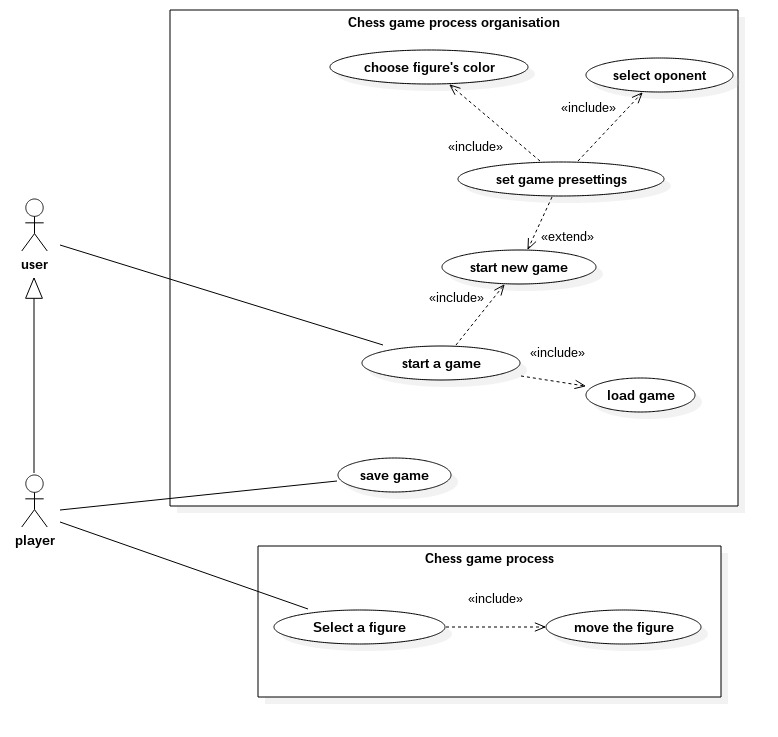
\includegraphics[scale=0.7]{../diagramms/UseCaseDia.jpg}
		\caption{UML-диаграмма вариантов использования приложения} 
		\label{pic:UseCaseDiagramm} % название для ссылок внутри кода
	\end{center}
\end{figure}

\subsection*{Вывод}
\addcontentsline{toc}{subsection}{Вывод}
Был получен навык работы с UML диаграммами, что позволило лучшее структуризировать проект.

\section*{Проектирование приложения,реализующего игру шахматы}
\addcontentsline{toc}{section}{Глава 2. Проектирование приложения,реализующего игру шахматы}

В проекте было выделено 5 подпроектов:
\begin{itemize}
\item Ядро - chessEngine
\item chessCUI - консольное приложение
\item chessGUI - графическое приложение
\item chessAI - искуственный интеллект
\item Тесты
\end{itemize}

На рис. \ref{pic:ProjectOrganisation} изображена UML - диаграмма компонентов, отображающая общую структуру проекта, разделение на подпроекты

\begin{figure}[H]
	\begin{center}
		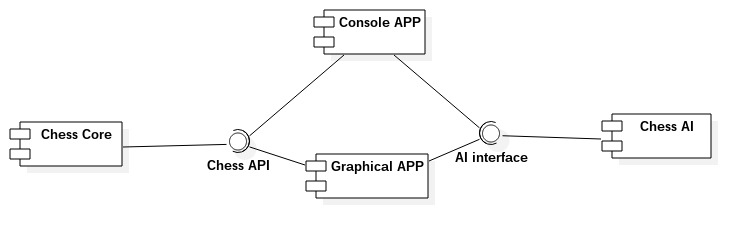
\includegraphics[scale=0.7]{../diagramms/component_dia.jpg}
		\caption{UML-диаграмма компонентов} 
		\label{pic:ProjectOrganisation} % название для ссылок внутри кода
	\end{center}
\end{figure}



\subsection*{chessEngine}
\addcontentsline{toc}{subsection}{chessEngine}
Ядро приложения, реализующее игровую логику.\\

\subsection*{chessEngine API}
\addcontentsline{toc}{subsection}{chessEngine API}
Интерфейс ядра предоставляет следующие возможности использования:
\begin{itemize}
\item\textbf{void chooseMyFigure(int x, int y);}\\
Позволяет выбрать по передаваемым координатам  фигуру, которой впоследствии будет выполнен ход\\
\item\textbf{void moveMyFigure(int x, int y);}\\
Позволяет переместить выбранную фигуру на указанную позицию\\
\item\textbf{myFigure* getMyFigure(int x, int y);}\\
Возвращает указатель на содержимое игровой доски на указанной позиции\\
\item\textbf{bool isFigureSelected();}\\
Возвращает TRUE если фигура уже выбрана и FALSE, если не выбрана\\
\end{itemize}

\subsection*{Тесты}
\addcontentsline{toc}{subsection}{Тесты}
Будут реализованы позже

\subsection*{Стандарты языка}
\addcontentsline{toc}{subsection}{Стандарты языка}
При создании приложения использовались:
\begin{itemize}
\item\textbf{c++98}\\
\item\textbf{c++11}\\
\end{itemize}

\subsection*{Компилятор}
\addcontentsline{toc}{subsection}{Компилятор}
\textbf{GCC 4.9.1}\\

\subsection*{Вывод}
\addcontentsline{toc}{subsection}{Вывод}
Был получен опыт работы с проектированием объектно-ориентированного приложения. 

\section*{Реализация игры шахматы}
\addcontentsline{toc}{section}{Глава 3. Реализация игры шахматы}

\subsection*{Среда разработки}
\addcontentsline{toc}{subsection}{Среда разработки}

\noindent\textbf{IDE:}Qt Creator 3.5.0 (opensource)\\
\textbf{OS:}Debian 3.14.1\\
\textbf{Документация:}Doxygen 1.8.8\\
\textbf{Компилятор:}GCC 4.9.1\\
\textbf{Анализатор:}Valgrind 3.10.0\\
\textbf{SVN:}Git 2.1.4

\subsection*{chessEngine}
\addcontentsline{toc}{subsection}{chessEngine}
Ядро содержит 18 классов, из которых 1 является интерфейсом ядра, 7 - исключения, 7 классов используется для представления фигур, один класс задаёт структуру клетки, и один класс задаёт структуру игральной доски.\\
\textbf{Основные классы:}\\
\begin{itemize}
\item\textbf{class myCell}\\
Класс, задающий структуру клетки на игральной доске\\
\item\textbf{class myFigure}\\
Абстрактный класс, задающий общее представление об объектах фигур. От него наследуются все остальные классы фигур\\
\item\textbf{class Pawn: public myFigure}\\
Класс для представления пешек. Содержит цвет и позицию фигуры. Наследуется от myFigure\\
\item\textbf{class Knight: public myFigure}\\
Класс для представления фигуры "Конь". Содержит цвет и позицию фигуры. Наследуется от myFigure\\
\item\textbf{class Rook: public myFigure}\\
Класс для представления Ладьи. Содержит цвет и позицию фигуры. Наследуется от myFigure\\
\item\textbf{class Bishop: public myFigure}\\
Класс для предсталения фигуры "Слон". Содержит цвет и позицию фигуры. Наследуется от myFigure\\
\item\textbf{class King: public myFigure}\\
Класс для представления фигуры "Король". Содержит цвет и позицию фигуры. Наследуется от myFigure\\
\item\textbf{class Queen: public myFigure}\\
Класс для представления ферзя. Содержит цвет и позицию фигуры. Наследуется от myFigure\\
\item\textbf{class BoardLogic}\\
Класс для представления игральной доски. Содержит двумерный массив указателей на фигуры\\
\item\textbf{class OutOfBoardException}\\
Исключение, генерируемое при попытке походить за границы доски\\
\item\textbf{class FigureNotSelectedException}\\
Исключение, генерируемое при попытке сделать ход, не выбрав фигуру\\
\item\textbf{class SameColorFigureException}\\
Исключение, генерируемое при поытке атаковать собственную фигуру\\
\item\textbf{class EmptyCellException}\\
Исключение, генерируемое при попытке выбрать пустую клетку\\
\item\textbf{class AgainstTheRulesException}\\
Исключение, генерируемое при попытке переместить фигуру не по правилам игры\\
\item\textbf{class WrongColorMoveException}\\
Исключение, генерируемое при попытке переместить фигуру не в свой ход\\
\item\textbf{class KingKilledException}\\
Исключение, генерируемое при взятии короля\\
\end{itemize}

\subsection*{chessCUI}
\addcontentsline{toc}{subsection}{chessCUI}
Содержит один класс \textbf{class Game}, реализующий консольное приложение.\\
На рис.\ref{pic:CUImenu} изображено меню консольного приложения.\\
\begin{figure}[H]
	\begin{center}
		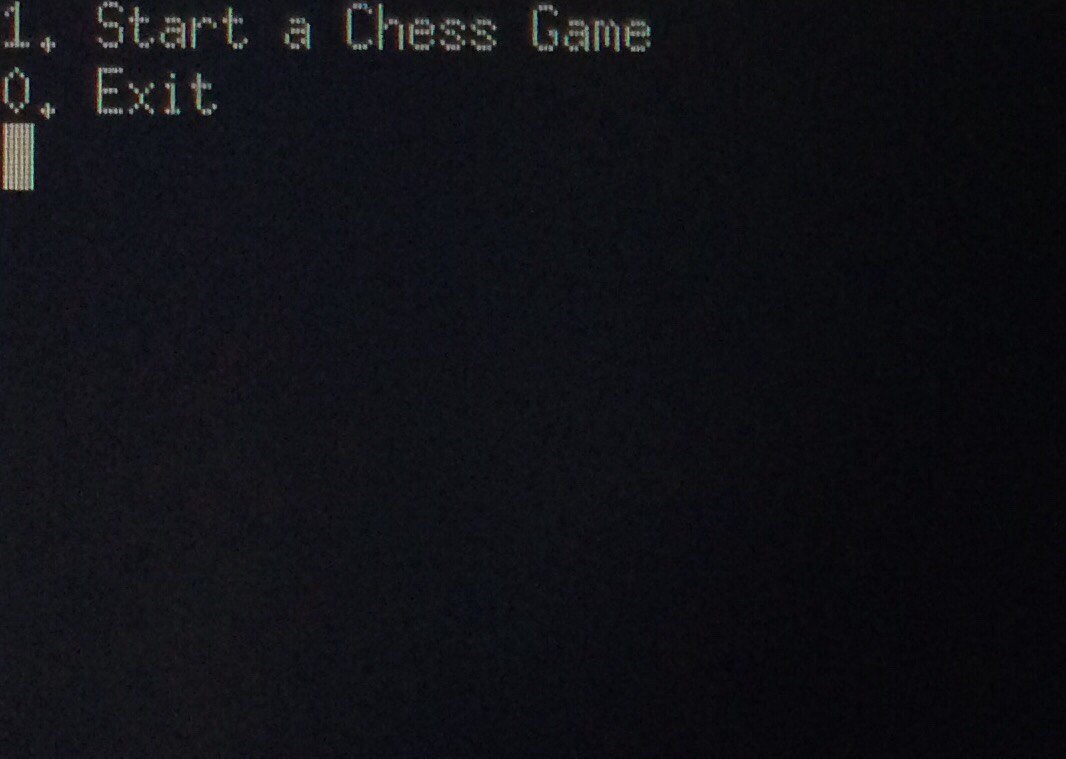
\includegraphics[scale=0.1]{pics/cuiMenu.jpg}
		\caption{Главное меню консольного приложения} 
		\label{pic:CUImenu} % название для ссылок внутри кода
	\end{center}
\end{figure}

На рис.\ref{pic:CUIdialog} показан пример обработки вводимых сообщений и реализация возможности сделать ход.\\
\begin{figure}[H]
	\begin{center}
		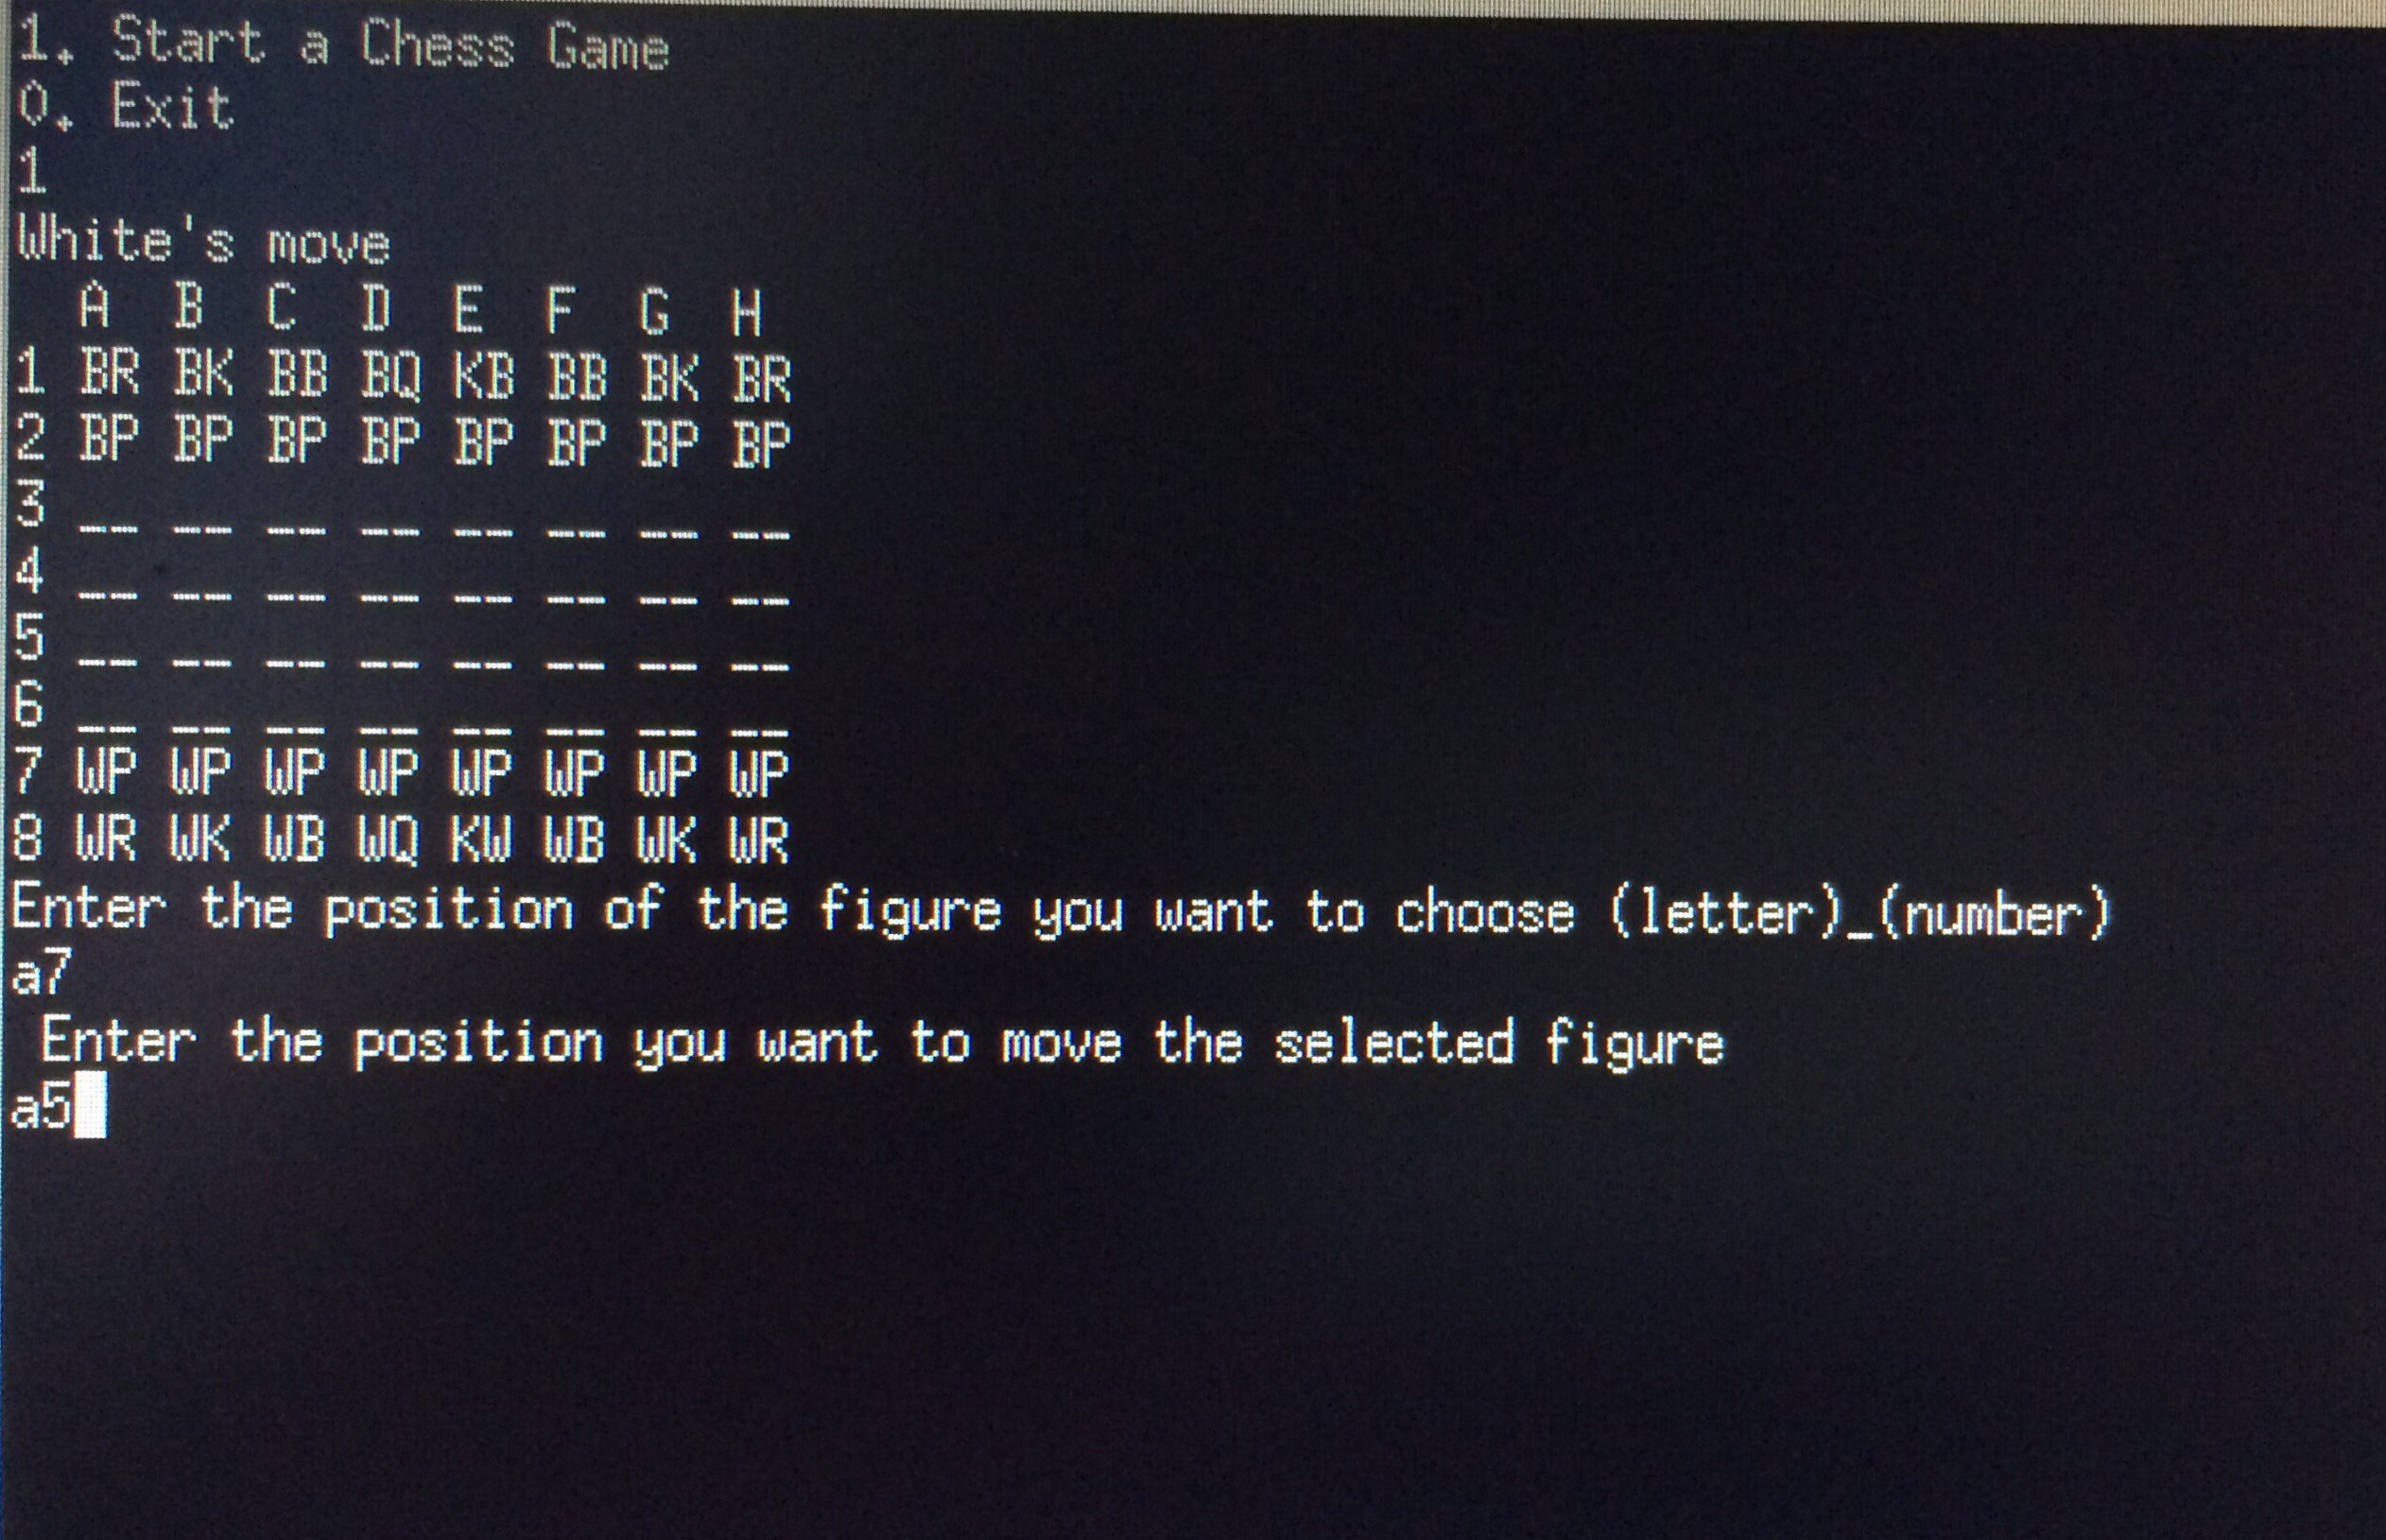
\includegraphics[scale=0.1]{pics/cui2.jpg}
		\caption{Обработка вводимых сообщений} 
		\label{pic:CUIdialog} % название для ссылок внутри кода
	\end{center}
\end{figure}

На рис.\ref{pic:CUIemptyCell} показано как обрабатывается исключению при попытке выбрать пустую клетку.\\
\begin{figure}[H]
	\begin{center}
		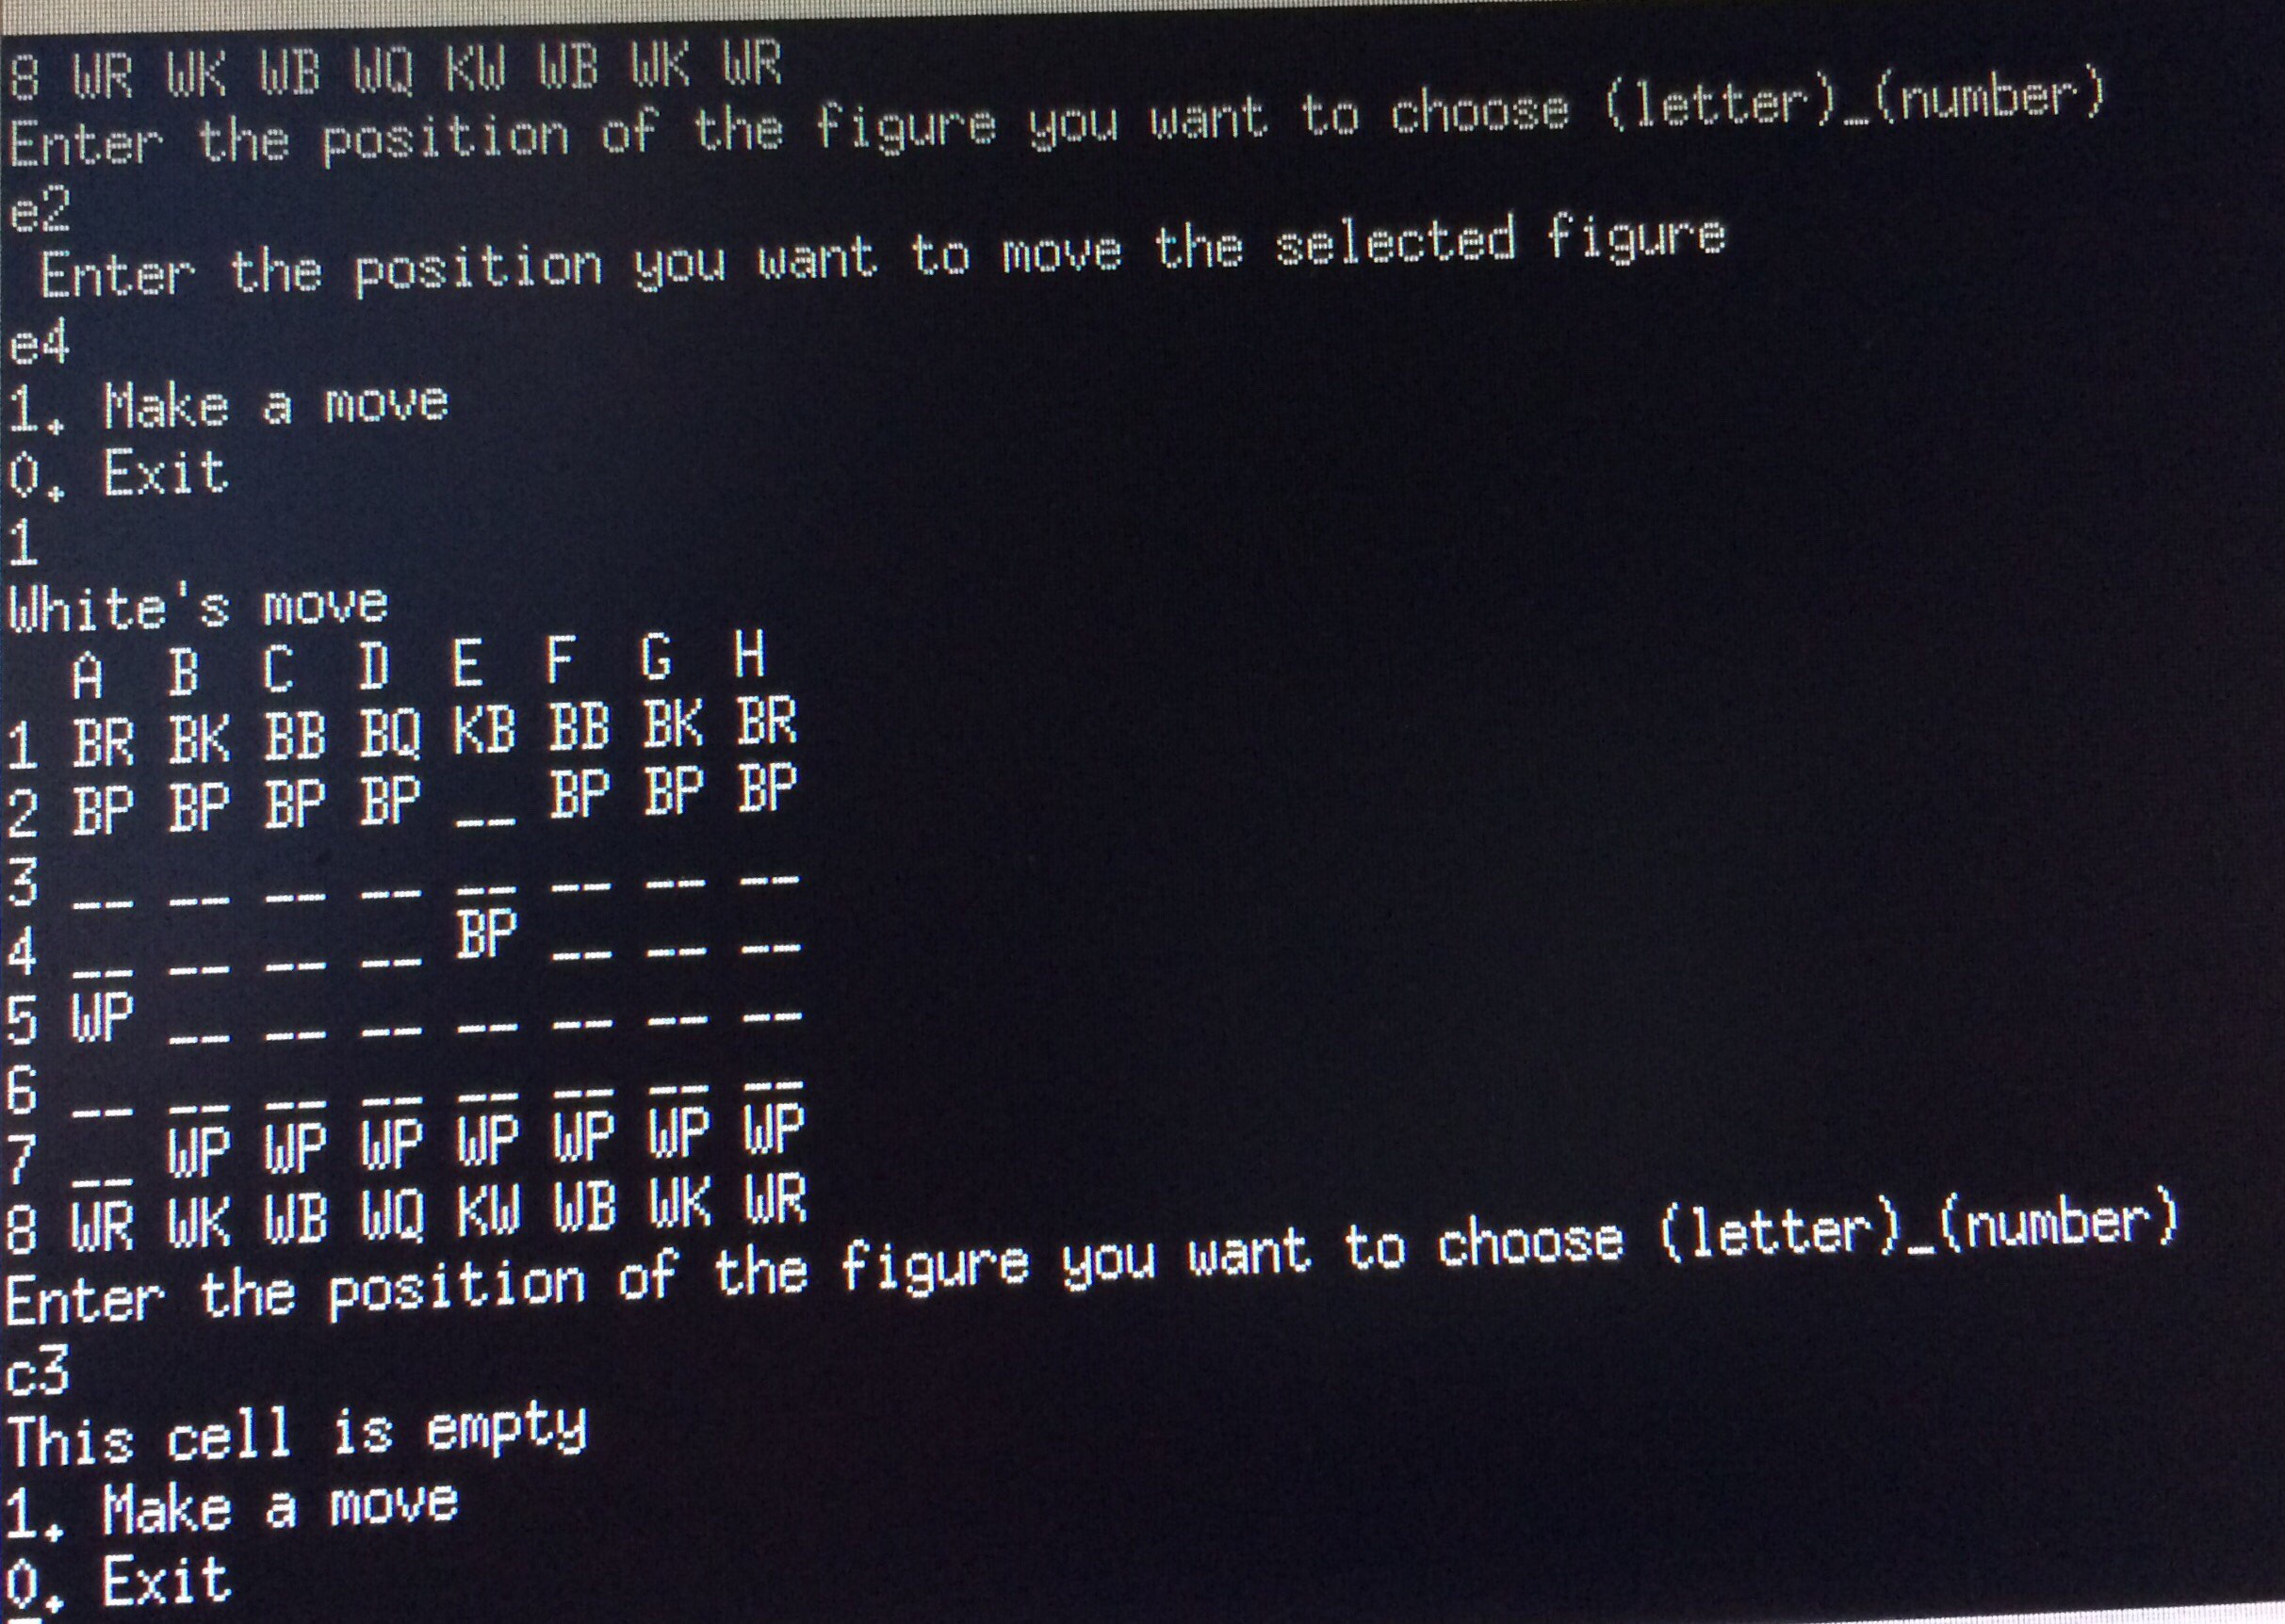
\includegraphics[scale=0.1]{pics/cui1.jpg}
		\caption{Сообщение о попытке выбрать пустую клетку} 
		\label{pic:CUIemptyCell} % название для ссылок внутри кода
	\end{center}
\end{figure}

\subsection*{chessGUI}
\addcontentsline{toc}{subsection}{chessGUI}
Содержит 3 класса для представления и отрисовки различных окон графического приложения:
\begin{itemize}
\item\textbf{class MainWindow: public QMainWindow}\\
Класс для отображения нужного виджета в соответствии с запросом пользователя. С помощью QStackedWidget контролирует, чтобы одновременно отображалось только одно окно\\
\item\textbf{class Dialog: public QDialog}\\
Класс для отображения начального меню\\
\item\textbf{class Board: public Qidget}\\
Класс для графического представления игральной доски с фигурами\\
\end{itemize}

На рис.\ref{pic:GUImenu} показано главное меню приложения, где пользователю предоставляется возможность начать игру, либо выйти.\\
\begin{figure}[H]
	\begin{center}
		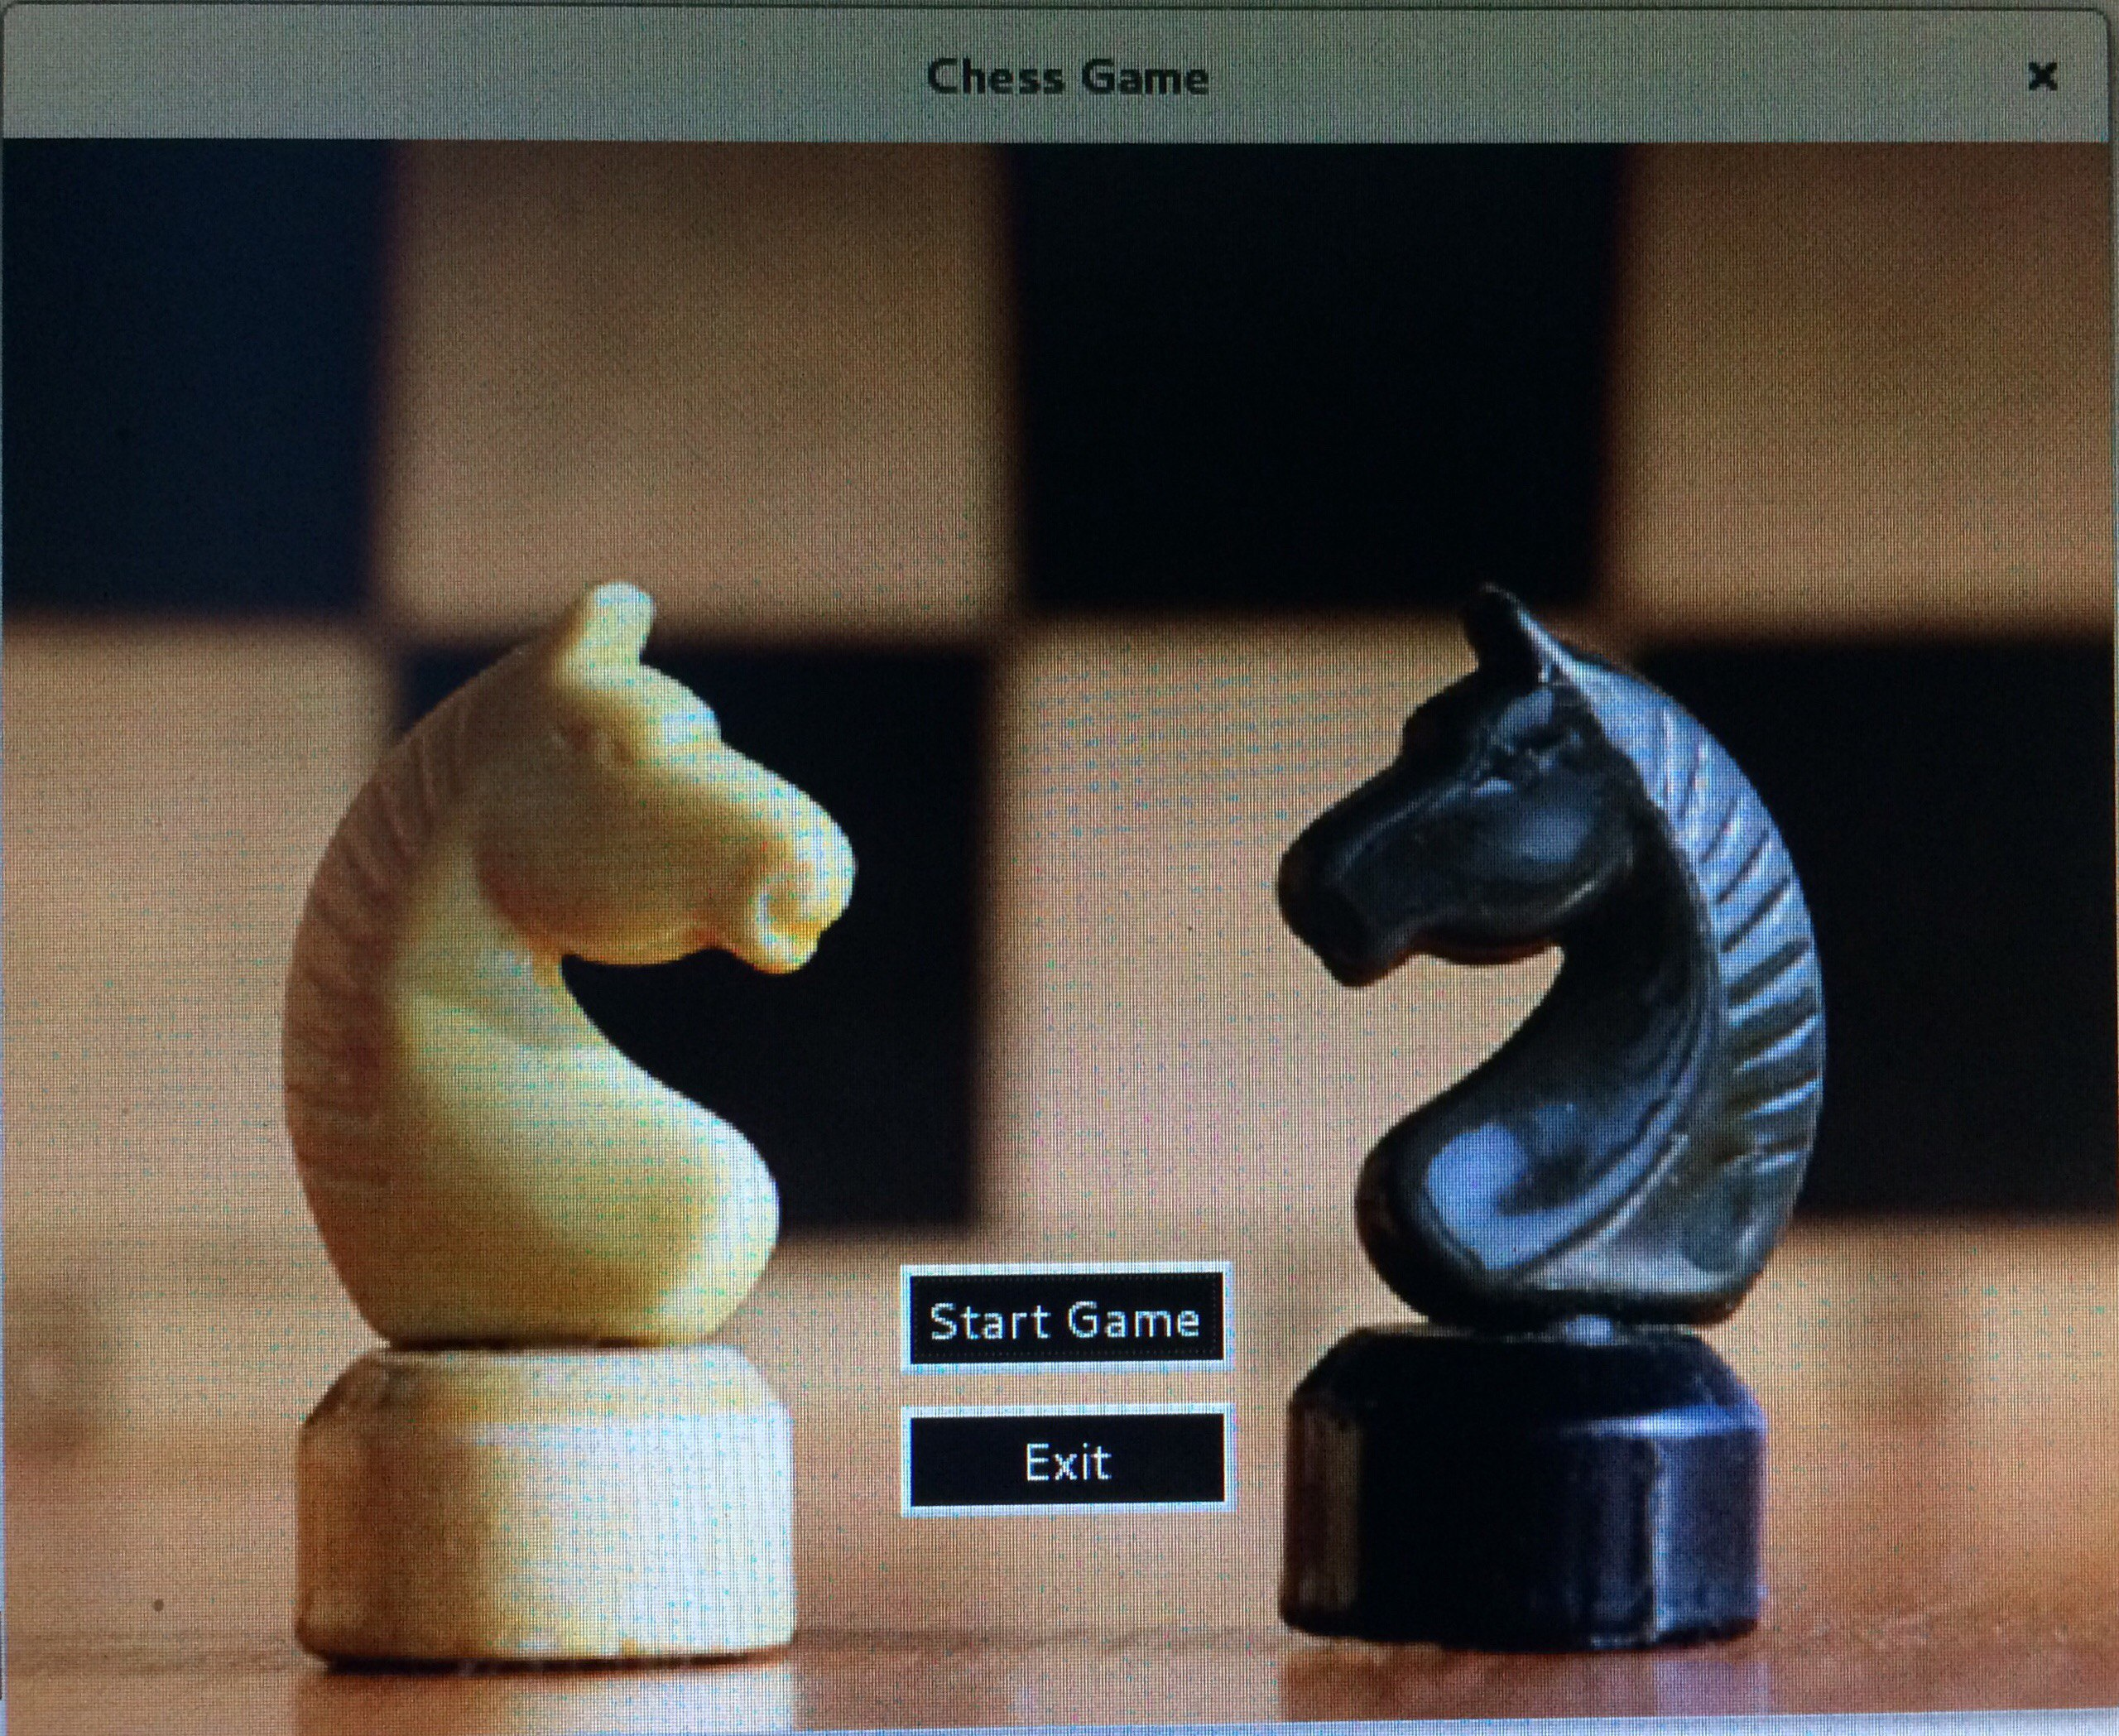
\includegraphics[scale=0.1]{pics/menuGui.jpg}
		\caption{Меню графического приложения} 
		\label{pic:GUImenu} % название для ссылок внутри кода
	\end{center}
\end{figure}

На рис.\ref{pic:GUIgameBoard} показано как отрисовывается игровое поля в самом начале игры.\\

\begin{figure}[H]
	\begin{center}
		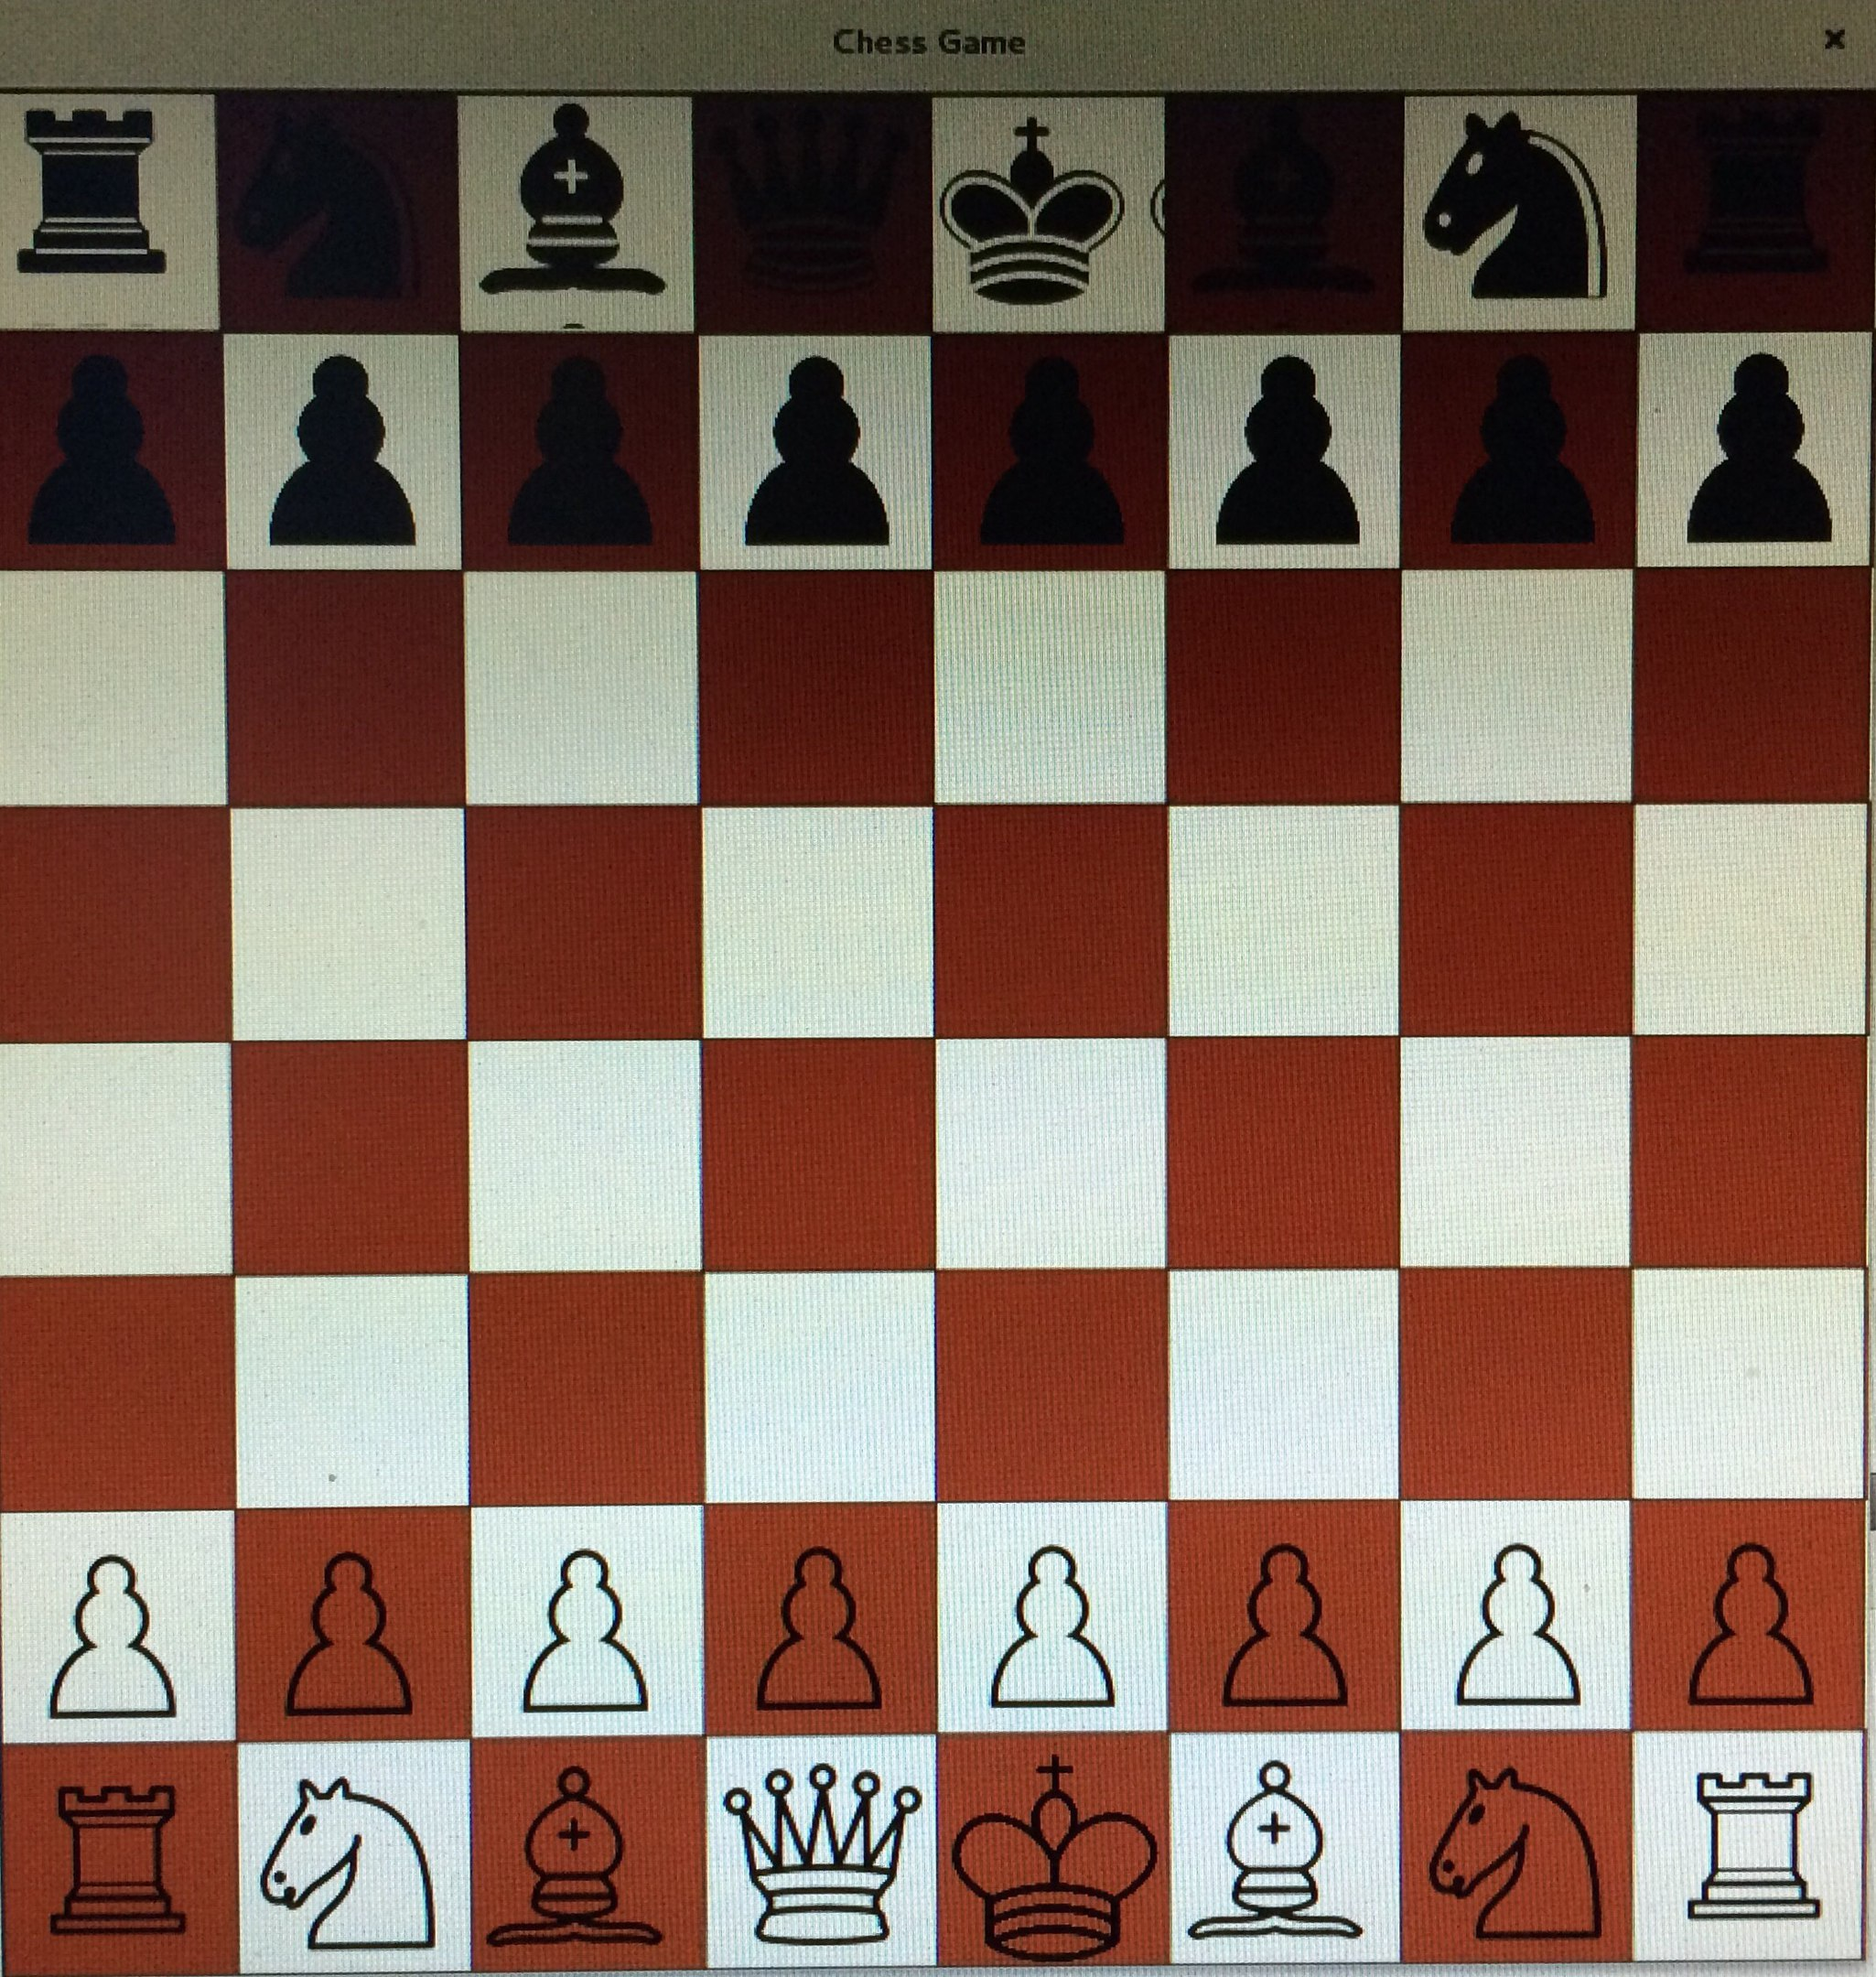
\includegraphics[scale=0.1]{pics/gui3.jpg}
		\caption{Отрисовка игрового поля} 
		\label{pic:GUIgameBoard} % название для ссылок внутри кода
	\end{center}
\end{figure}

На рис.\ref{pic:GUIwrongMoveMessege} показано сообщение, возникающее при попытке походить не в свой ход.\\
\begin{figure}[H]
	\begin{center}
		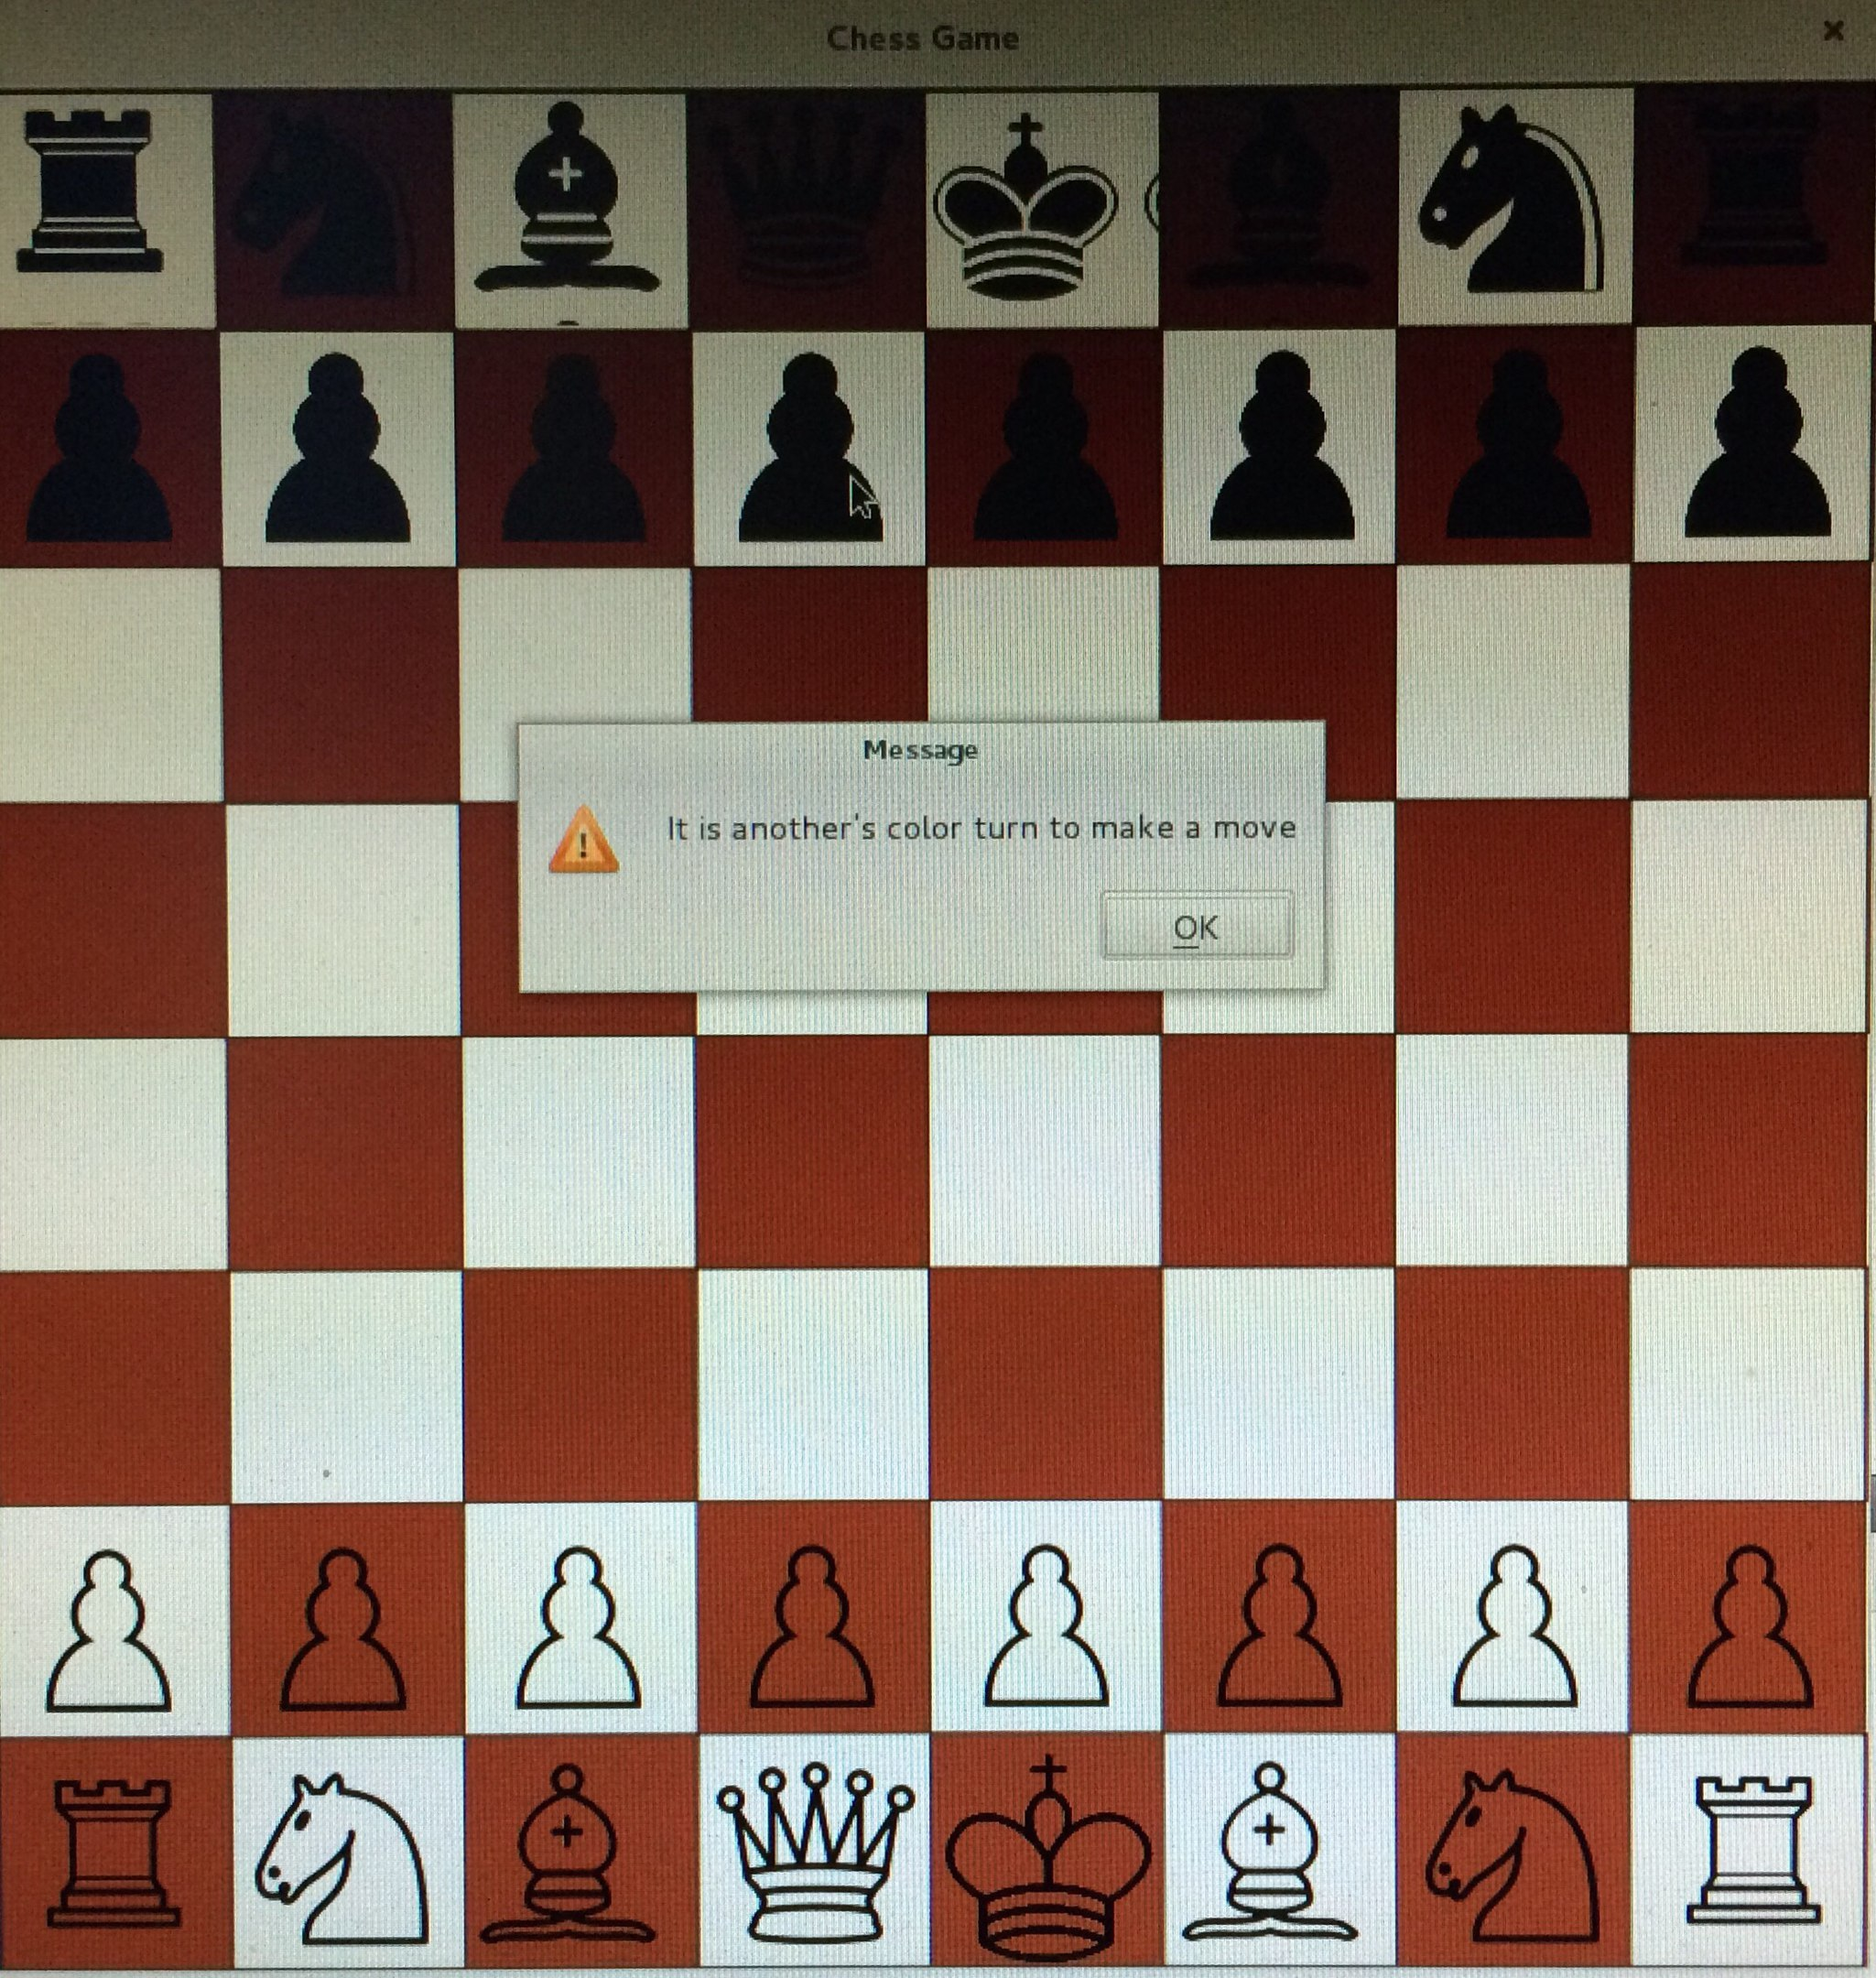
\includegraphics[scale=0.1]{pics/gui2.jpg}
		\caption{Сообщение о нарушении очерёдности хода в игре} 
		\label{pic:GUIwrongMoveMessege} % название для ссылок внутри кода
	\end{center}
\end{figure}

На рис.\ref{pic:GUIgameOverMessege} показано сообщение, которое высвечивается при взятии одного из королей.\\
\begin{figure}[H]
	\begin{center}
		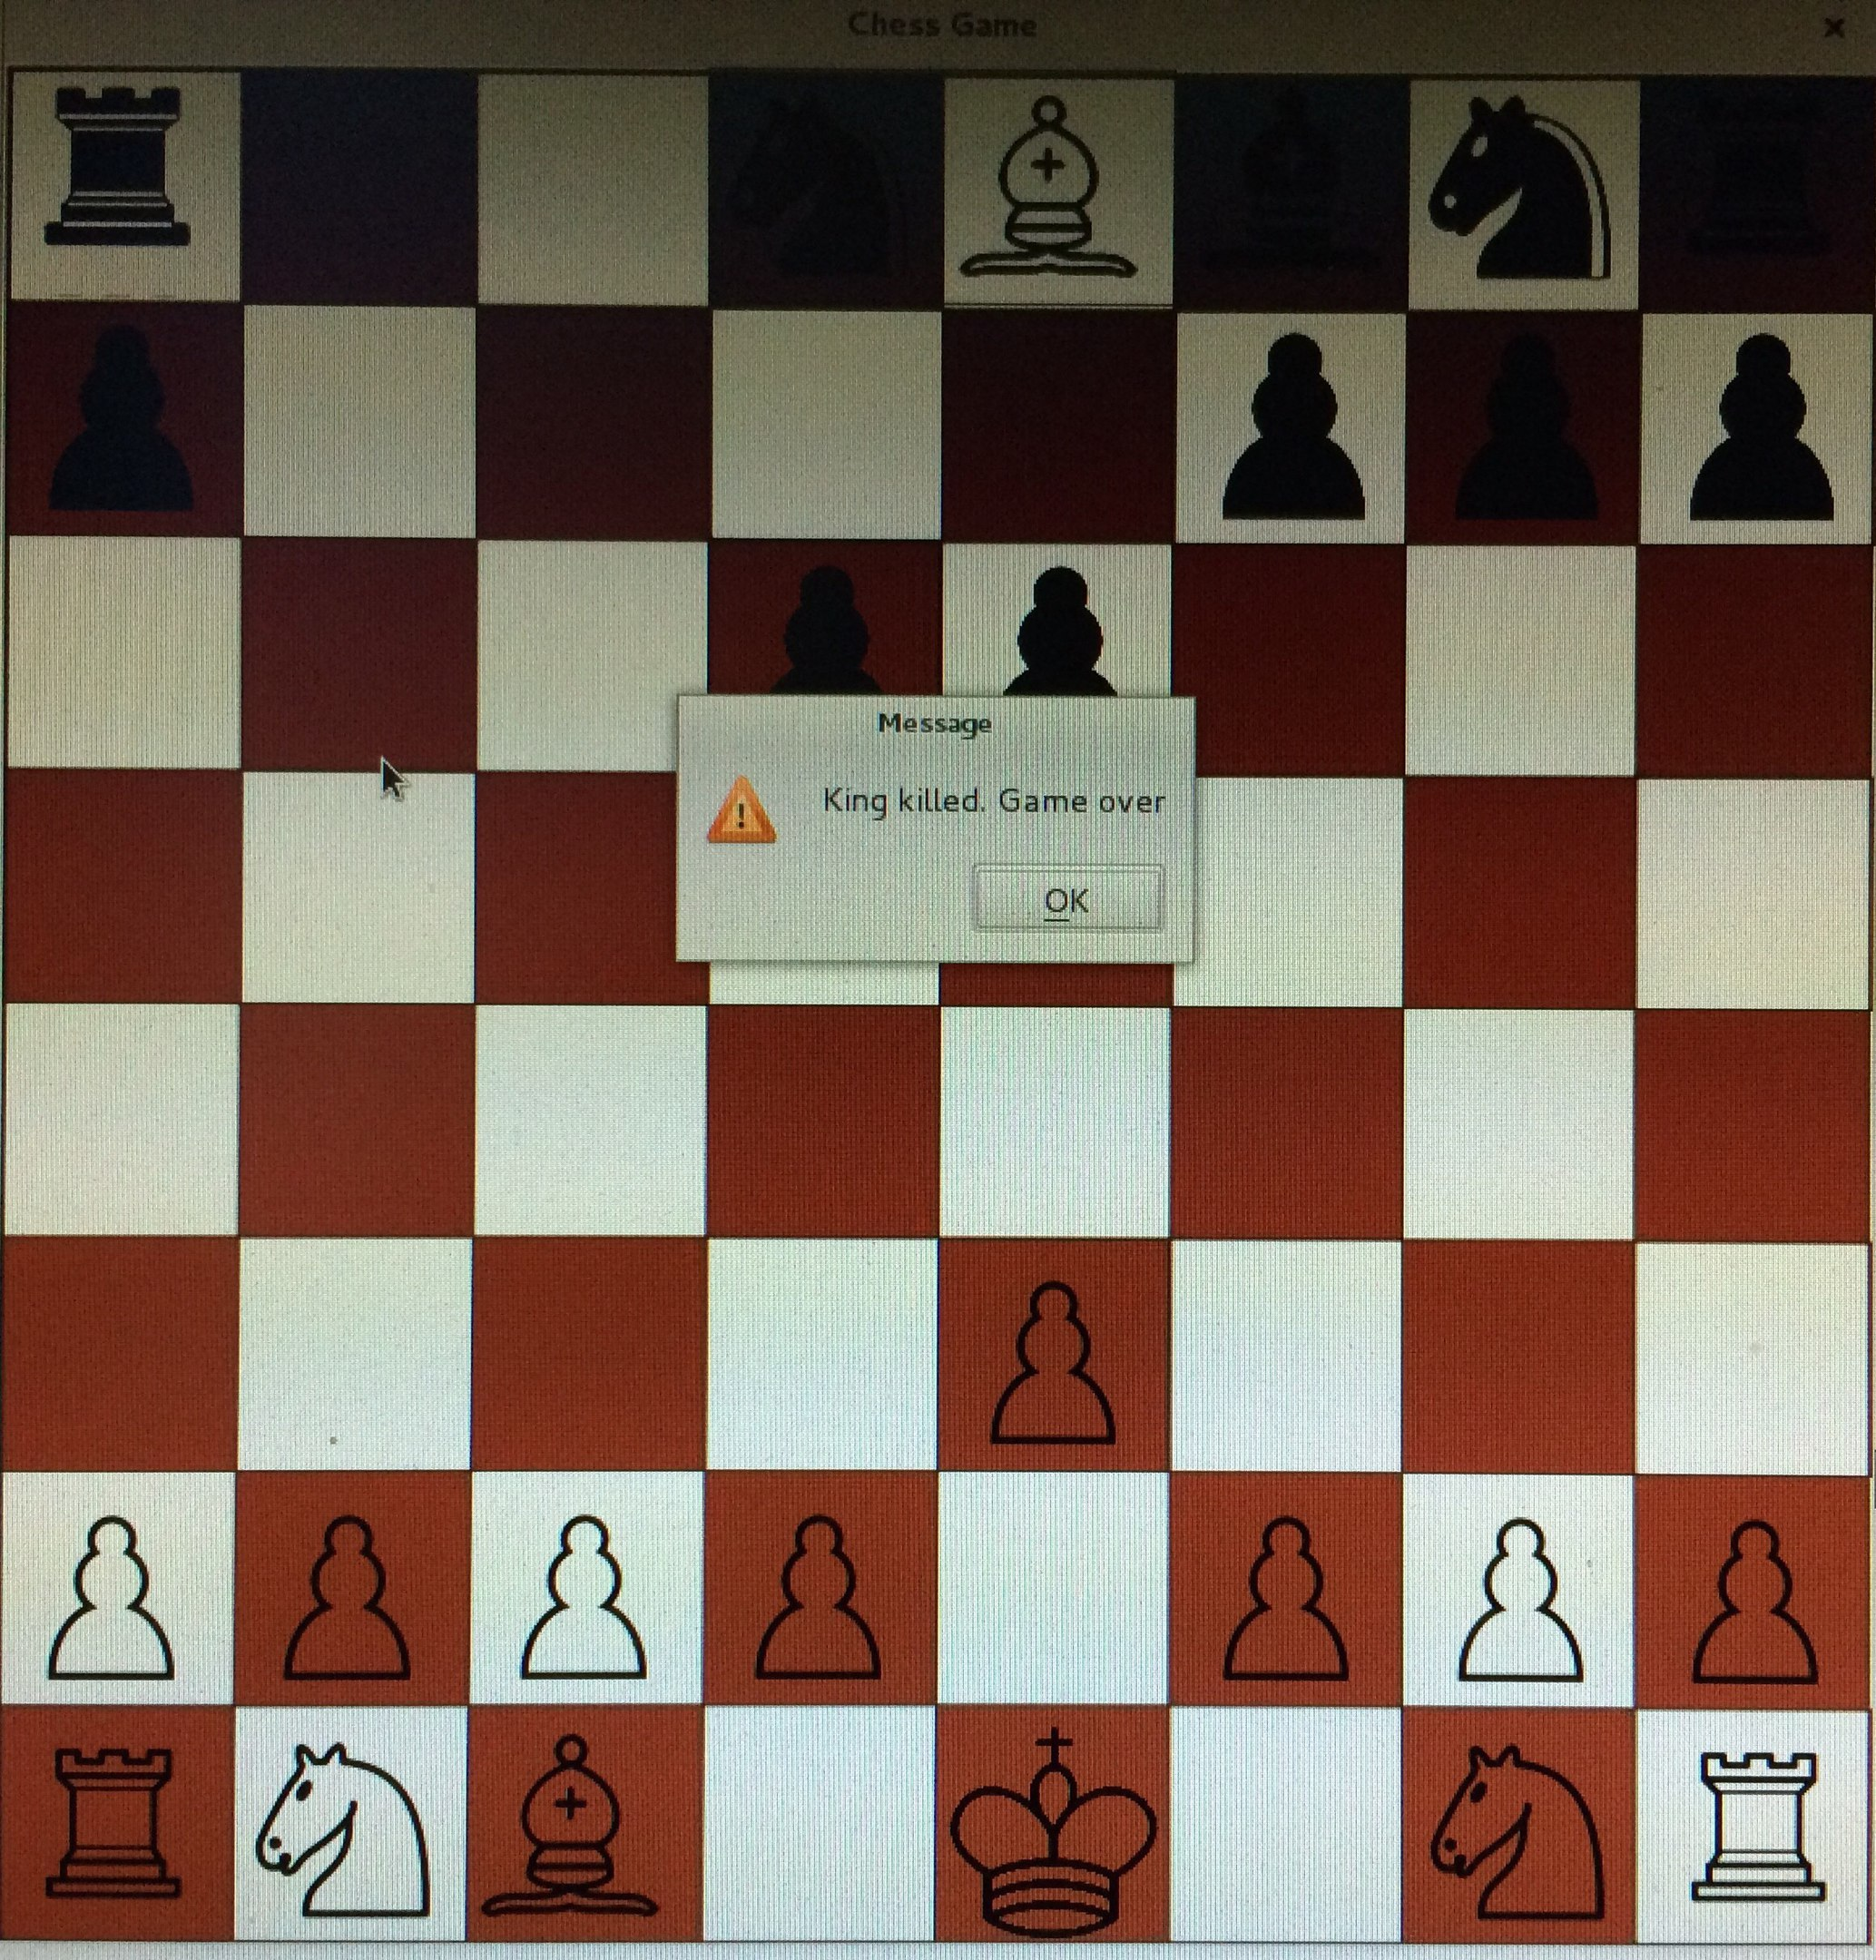
\includegraphics[scale=0.1]{pics/gui1.jpg}
		\caption{Сообщение об окончании игры} 
		\label{pic:GUIgameOverMessege} % название для ссылок внутри кода
	\end{center}
\end{figure}

\subsection{Листинг}

%\captionof{lstlisting}{hell\_o.c} % для печати символ '_' требует выходной символ '\'
%\lstinputlisting[label=code:hello]{listings/hell_o.c}
%\parindent=1cm % командна \lstinputlisting сбивает параментры отступа
Текст без отступа (следует за вставкой)

Новый параграф

\noindent Новый параграф с принудительно выключенным отступом



\section{Выводы}
\LaTeX\ удобен для создания отчётов, так как сам следит за нумерацией таблиц, рисунков, листингов и отсылок к ним (так, например, здесь всегда будет указан номер рисунка "sample" не зависимо от того, какой он (1,2 или другой) - это рисунок \ref{pic:pic_name}). Не менее важно что весь документ оформлен в едином стиле, а исходные материалы подключаются к отчёту, а не хранятся в нём. Всё это позволяет легко получить качественный отчёт без дополнительных трат на его офрмление.

Исключения, пожалуй, составляют таблицы, так как их значительно сложнее создавать кодом, нежели в графическом редакторе. Но здесь никто не запрещает использовать визуальные средства создания таблиц для \LaTeX\ .
\end{document}
